\chapter{Tasoitettu analyysi}

\index{tasoitettu analyysi@tasoitettu analyysi}

Monen algoritmin aikavaativuuden pystyy laskemaan
suoraan katsomalla algoritmin rakennetta:
mitä silmukoita algoritmissa on ja miten monta
kertaa niitä suoritetaan.
Joskus kuitenkaan näin suoraviivainen analyysi ei
riitä antamaan todellista kuvaa algoritmin tehokkuudesta.

\key{Tasoitettu analyysi} soveltuu sellaisten
algoritmien analyysiin, joiden osana on jokin operaatio,
jonka ajankäyttö vaihtelee.
Ideana on tarkastella yksittäisen operaation
sijasta kaikkia operaatioita algoritmin
aikana ja laskea niiden ajankäytölle yhteinen raja.

\section{Kaksi osoitinta}

\index{kaksi osoitinta@kaksi osoitinta}

Kahden osoittimen tekniikka on taulukon käsittelyssä
käytettävä tekniikka, jossa taulukkoa käydään läpi
kahden osoittimen avulla.
Molemmat osoittimet liikkuvat algoritmin aikana,
mutta rajoituksena on, että ne voivat liikkua vain
yhteen suuntaan, mikä takaa, että algoritmi toimii tehokkaasti.

Tutustumme seuraavaksi kahden osoittimen tekniikkaan
kahden esimerkkitehtävän kautta.

\subsubsection{Esimerkki 1}

\begin{task}
Annettuna on taulukko, jossa on $n$ positiivista kokonaislukua.
Tehtäväsi on tutkia, onko taulukossa väliä,
jossa lukujen summa on $x$.
\end{task}

Ideana on käydä taulukkoa läpi kahden osoittimen
avulla, jotka rajaavat välin taulukosta.
Joka vuorolla vasen osoitin liikkuu
yhden askeleen eteenpäin, kun taas oikea osoitin
liikkuu niin kauan eteenpäin kuin summa on enintään $x$.
Jos välin summaksi tulee tarkalleen $x$, ratkaisu on löytynyt.

Tarkastellaan esimerkkinä algoritmin toimintaa
seuraavassa taulukossa, kun tavoitteena on muodostaa summa $x=8$:
\begin{center}
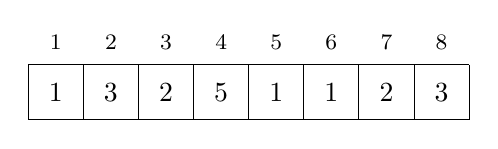
\begin{tikzpicture}[scale=0.7]
\draw (0,0) grid (8,1);

\node at (0.5,0.5) {$1$};
\node at (1.5,0.5) {$3$};
\node at (2.5,0.5) {$2$};
\node at (3.5,0.5) {$5$};
\node at (4.5,0.5) {$1$};
\node at (5.5,0.5) {$1$};
\node at (6.5,0.5) {$2$};
\node at (7.5,0.5) {$3$};

\footnotesize
\node at (0.5,1.4) {$1$};
\node at (1.5,1.4) {$2$};
\node at (2.5,1.4) {$3$};
\node at (3.5,1.4) {$4$};
\node at (4.5,1.4) {$5$};
\node at (5.5,1.4) {$6$};
\node at (6.5,1.4) {$7$};
\node at (7.5,1.4) {$8$};
\end{tikzpicture}
\end{center}

Aluksi osoittimet rajaavat taulukosta välin,
jonka summa on $1+3+2=6$.
Väli ei voi olla tätä suurempi,
koska seuraava luku 5 veisi summan yli $x$:n.

\begin{center}
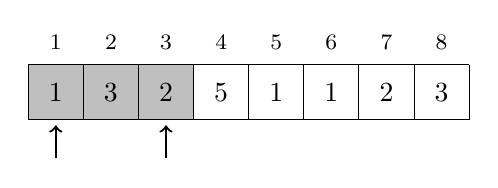
\begin{tikzpicture}[scale=0.7]
\fill[color=lightgray] (0,0) rectangle (3,1);
\draw (0,0) grid (8,1);

\node at (0.5,0.5) {$1$};
\node at (1.5,0.5) {$3$};
\node at (2.5,0.5) {$2$};
\node at (3.5,0.5) {$5$};
\node at (4.5,0.5) {$1$};
\node at (5.5,0.5) {$1$};
\node at (6.5,0.5) {$2$};
\node at (7.5,0.5) {$3$};

\draw[thick,->] (0.5,-0.7) -- (0.5,-0.1);
\draw[thick,->] (2.5,-0.7) -- (2.5,-0.1);

\footnotesize
\node at (0.5,1.4) {$1$};
\node at (1.5,1.4) {$2$};
\node at (2.5,1.4) {$3$};
\node at (3.5,1.4) {$4$};
\node at (4.5,1.4) {$5$};
\node at (5.5,1.4) {$6$};
\node at (6.5,1.4) {$7$};
\node at (7.5,1.4) {$8$};
\end{tikzpicture}
\end{center}

Seuraavaksi vasen osoitin siirtyy askeleen eteenpäin.
Oikea osoitin säilyy paikallaan, koska muuten
summa kasvaisi liian suureksi.

\begin{center}
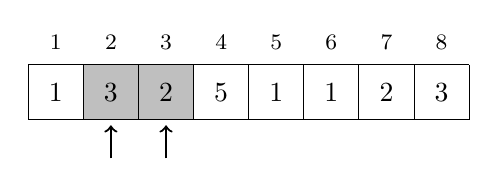
\begin{tikzpicture}[scale=0.7]
\fill[color=lightgray] (1,0) rectangle (3,1);
\draw (0,0) grid (8,1);

\node at (0.5,0.5) {$1$};
\node at (1.5,0.5) {$3$};
\node at (2.5,0.5) {$2$};
\node at (3.5,0.5) {$5$};
\node at (4.5,0.5) {$1$};
\node at (5.5,0.5) {$1$};
\node at (6.5,0.5) {$2$};
\node at (7.5,0.5) {$3$};

\draw[thick,->] (1.5,-0.7) -- (1.5,-0.1);
\draw[thick,->] (2.5,-0.7) -- (2.5,-0.1);

\footnotesize
\node at (0.5,1.4) {$1$};
\node at (1.5,1.4) {$2$};
\node at (2.5,1.4) {$3$};
\node at (3.5,1.4) {$4$};
\node at (4.5,1.4) {$5$};
\node at (5.5,1.4) {$6$};
\node at (6.5,1.4) {$7$};
\node at (7.5,1.4) {$8$};
\end{tikzpicture}
\end{center}

Vasen osoitin siirtyy taas askeleen eteenpäin
ja tällä kertaa oikea osoitin siirtyy kolme askelta
eteenpäin. Muodostuu summa $2+5+1=8$ eli taulukosta
on löytynyt väli, jonka lukujen summa on $x$.

\begin{center}
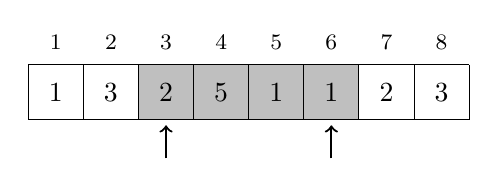
\begin{tikzpicture}[scale=0.7]
\fill[color=lightgray] (2,0) rectangle (6,1);
\draw (0,0) grid (8,1);

\node at (0.5,0.5) {$1$};
\node at (1.5,0.5) {$3$};
\node at (2.5,0.5) {$2$};
\node at (3.5,0.5) {$5$};
\node at (4.5,0.5) {$1$};
\node at (5.5,0.5) {$1$};
\node at (6.5,0.5) {$2$};
\node at (7.5,0.5) {$3$};

\draw[thick,->] (2.5,-0.7) -- (2.5,-0.1);
\draw[thick,->] (5.5,-0.7) -- (5.5,-0.1);

\footnotesize
\node at (0.5,1.4) {$1$};
\node at (1.5,1.4) {$2$};
\node at (2.5,1.4) {$3$};
\node at (3.5,1.4) {$4$};
\node at (4.5,1.4) {$5$};
\node at (5.5,1.4) {$6$};
\node at (6.5,1.4) {$7$};
\node at (7.5,1.4) {$8$};
\end{tikzpicture}
\end{center}

Algoritmin toteutus näyttää seuraavalta:

\begin{lstlisting}
int s = 0, b = 0;
for (int a = 1; a <= n; a++) {
    while (b<n && s+t[b+1] <= x) {
        b++;
        s += t[b];
    }
    if (s == x) {
        // ratkaisu löytyi
    }
    s -= t[a];
}
\end{lstlisting}

Muuttujat $a$ ja $b$ sisältävät vasemman ja oikean
osoittimen kohdan.
Muuttuja $s$ taas laskee lukujen summan välillä.
Joka askeleella $a$ liikkuu askeleen eteenpäin
ja $b$ liikkuu niin kauan kuin summa on enintään $x$.

Algoritmin aikavaativuus riippuu siitä,
kauanko \texttt{while}-silmukan suoritus vie aikaa.
Tämä vaihtelee, koska oikea osoitin voi liikkua
minkä tahansa matkan eteenpäin taulukossa.
Kuitenkin oikea osoitin liikkuu \textit{yhteensä}
$O(n)$ askelta algoritmin aikana, koska se voi
liikkua vain eteenpäin.

Koska sekä vasen että oikea osoitin liikkuvat
$O(n)$ askelta algoritmin aikana,
algoritmin aikavaativuus on $O(n)$.

\subsubsection{Esimerkki 2}

\begin{task}
Annettuna on taulukko, jossa on $n$ kokonaislukua.
Tehtäväsi on tutkia, voiko taulukosta valita kaksi lukua
niin, että niiden summa on $x$.
\end{task}

Tämänkin tehtävän voi ratkaista kahden osoittimen
tekniikalla, kuitenkin niin,
että osoittimet liikkuvat eri suuntiin.
Ideana on järjestää ensin taulukon luvut
pienimmästä suurimpaan ja
sitten käydä taulukkoa läpi kahdella osoittimella,
jotka lähtevät liikkelle sen molemmista päistä.

Vasen osoitin aloittaa taulukon alusta ja
liikkuu joka vaiheessa askeleen eteenpäin.
Oikea osoitin taas aloittaa taulukon lopusta
ja peruuttaa niin kauan, kunnes osoitinten
määrittämän välin lukujen summa on enintään $x$.
Jos summa on tarkalleen $x$, ratkaisu on löytynyt.

Tarkastellaan esimerkkinä algoritmin toimintaa
seuraavassa taulukossa, kun tavoitteena on muodostaa
summa $x=12$:
\begin{center}
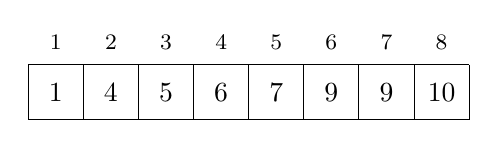
\begin{tikzpicture}[scale=0.7]
\draw (0,0) grid (8,1);

\node at (0.5,0.5) {$1$};
\node at (1.5,0.5) {$4$};
\node at (2.5,0.5) {$5$};
\node at (3.5,0.5) {$6$};
\node at (4.5,0.5) {$7$};
\node at (5.5,0.5) {$9$};
\node at (6.5,0.5) {$9$};
\node at (7.5,0.5) {$10$};

\footnotesize
\node at (0.5,1.4) {$1$};
\node at (1.5,1.4) {$2$};
\node at (2.5,1.4) {$3$};
\node at (3.5,1.4) {$4$};
\node at (4.5,1.4) {$5$};
\node at (5.5,1.4) {$6$};
\node at (6.5,1.4) {$7$};
\node at (7.5,1.4) {$8$};
\end{tikzpicture}
\end{center}

Seuraavassa on algoritmin aloitustilanne.
Lukujen summa on $1+10=11$, joka on pienempi
kuin $x$:n arvo.

\begin{center}
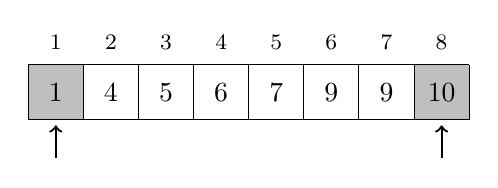
\begin{tikzpicture}[scale=0.7]
\fill[color=lightgray] (0,0) rectangle (1,1);
\fill[color=lightgray] (7,0) rectangle (8,1);
\draw (0,0) grid (8,1);

\node at (0.5,0.5) {$1$};
\node at (1.5,0.5) {$4$};
\node at (2.5,0.5) {$5$};
\node at (3.5,0.5) {$6$};
\node at (4.5,0.5) {$7$};
\node at (5.5,0.5) {$9$};
\node at (6.5,0.5) {$9$};
\node at (7.5,0.5) {$10$};

\draw[thick,->] (0.5,-0.7) -- (0.5,-0.1);
\draw[thick,->] (7.5,-0.7) -- (7.5,-0.1);

\footnotesize
\node at (0.5,1.4) {$1$};
\node at (1.5,1.4) {$2$};
\node at (2.5,1.4) {$3$};
\node at (3.5,1.4) {$4$};
\node at (4.5,1.4) {$5$};
\node at (5.5,1.4) {$6$};
\node at (6.5,1.4) {$7$};
\node at (7.5,1.4) {$8$};
\end{tikzpicture}
\end{center}

Seuraavaksi vasen osoitin liikkuu askeleen eteenpäin.
Oikea osoitin peruuttaa kolme askelta, minkä jälkeen
summana on $4+7=11$.

\begin{center}
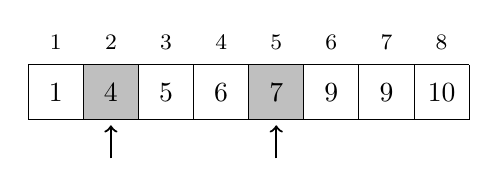
\begin{tikzpicture}[scale=0.7]
\fill[color=lightgray] (1,0) rectangle (2,1);
\fill[color=lightgray] (4,0) rectangle (5,1);
\draw (0,0) grid (8,1);

\node at (0.5,0.5) {$1$};
\node at (1.5,0.5) {$4$};
\node at (2.5,0.5) {$5$};
\node at (3.5,0.5) {$6$};
\node at (4.5,0.5) {$7$};
\node at (5.5,0.5) {$9$};
\node at (6.5,0.5) {$9$};
\node at (7.5,0.5) {$10$};

\draw[thick,->] (1.5,-0.7) -- (1.5,-0.1);
\draw[thick,->] (4.5,-0.7) -- (4.5,-0.1);

\footnotesize
\node at (0.5,1.4) {$1$};
\node at (1.5,1.4) {$2$};
\node at (2.5,1.4) {$3$};
\node at (3.5,1.4) {$4$};
\node at (4.5,1.4) {$5$};
\node at (5.5,1.4) {$6$};
\node at (6.5,1.4) {$7$};
\node at (7.5,1.4) {$8$};
\end{tikzpicture}
\end{center}

Sitten vasen osoitin siirtyy jälleen askeleen eteenpäin.
Oikea osoitin pysyy paikallaan ja ratkaisu $5+7=12$ on löytynyt.

\begin{center}
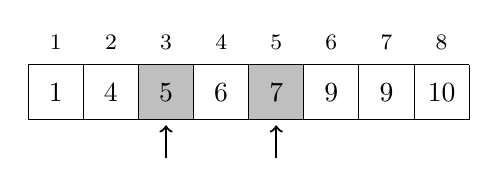
\begin{tikzpicture}[scale=0.7]
\fill[color=lightgray] (2,0) rectangle (3,1);
\fill[color=lightgray] (4,0) rectangle (5,1);
\draw (0,0) grid (8,1);

\node at (0.5,0.5) {$1$};
\node at (1.5,0.5) {$4$};
\node at (2.5,0.5) {$5$};
\node at (3.5,0.5) {$6$};
\node at (4.5,0.5) {$7$};
\node at (5.5,0.5) {$9$};
\node at (6.5,0.5) {$9$};
\node at (7.5,0.5) {$10$};

\draw[thick,->] (2.5,-0.7) -- (2.5,-0.1);
\draw[thick,->] (4.5,-0.7) -- (4.5,-0.1);

\footnotesize
\node at (0.5,1.4) {$1$};
\node at (1.5,1.4) {$2$};
\node at (2.5,1.4) {$3$};
\node at (3.5,1.4) {$4$};
\node at (4.5,1.4) {$5$};
\node at (5.5,1.4) {$6$};
\node at (6.5,1.4) {$7$};
\node at (7.5,1.4) {$8$};
\end{tikzpicture}
\end{center}

Algoritmin alussa taulukon järjestäminen vie
aikaa $O(n \log n)$.
Tämän jälkeen vasen osoitin liikkuu $O(n)$ askelta
eteenpäin ja oikea osoitin liikkuu $O(n)$ askelta
taaksepäin, mihin kuluu aikaa $O(n)$.
Algoritmin kokonaisaikavaativuus on siis $O(n \log n)$.

Huomaa, että tehtävän voi ratkaista myös 
toisella tavalla ajassa
$O(n \log n)$ binäärihaun avulla.
Tässä ratkaisussa jokaiselle taulukon luvulle
etsitään binäärihaulla toista lukua niin,
että lukujen summa olisi yhteensä $x$.
Binäärihaku suoritetaan $n$ kertaa ja
jokainen binäärihaku vie aikaa $O(\log n)$.

\section{Lähin pienempi edeltäjä}

\index{lzhin pienempi edeltxjx@lähin pienempi edeltäjä}

Tasoitetun analyysin avulla arvioidaan usein
tietorakenteeseen tehtävien operaatioiden määrää.
Algoritmin operaatiot voivat jakautua epätasaisesti
niin, että useimmat operaatiot tehdään tietyssä
algoritmin vaiheessa ja muuten niitä tehdään vähän.
Näin on seuraavassa tehtävässä:

\begin{task}
Annettuna on taulukko, jossa on $n$ lukua.
Tehtäväsi on etsiä jokaiselle luvulle
sitä lähinnä oleva pienempi luku
taulukon alkuosassa
tai todeta, että tällaista lukua ei ole olemassa.
\end{task}

Tehokas ratkaisu tehtävään on käydä
taulukko läpi alusta loppuun ja pitää samalla yllä ketjua,
jonka ensimmäinen luku on käsiteltävä taulukon luku
ja jokainen seuraava luku on luvun lähin
pienempi edeltäjä.
Jos ketjussa on vain yksi luku,
käsiteltävällä luvulla ei ole pienempää edeltäjää.

Joka askeleella ketjun alusta poistetaan lukuja
niin kauan, kunnes ketjun ensimmäinen luku on 
pienempi kuin käsiteltävä taulukon luku tai ketju on tyhjä.
Tämän jälkeen käsiteltävä luku lisätään ketjun alkuun.

Tarkastellaan esimerkkinä algoritmin toimintaa
seuraavassa taulukossa:

\begin{center}
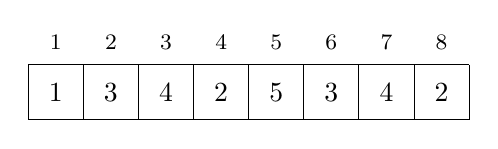
\begin{tikzpicture}[scale=0.7]
\draw (0,0) grid (8,1);

\node at (0.5,0.5) {$1$};
\node at (1.5,0.5) {$3$};
\node at (2.5,0.5) {$4$};
\node at (3.5,0.5) {$2$};
\node at (4.5,0.5) {$5$};
\node at (5.5,0.5) {$3$};
\node at (6.5,0.5) {$4$};
\node at (7.5,0.5) {$2$};

\footnotesize
\node at (0.5,1.4) {$1$};
\node at (1.5,1.4) {$2$};
\node at (2.5,1.4) {$3$};
\node at (3.5,1.4) {$4$};
\node at (4.5,1.4) {$5$};
\node at (5.5,1.4) {$6$};
\node at (6.5,1.4) {$7$};
\node at (7.5,1.4) {$8$};
\end{tikzpicture}
\end{center}
Aluksi luvut 1, 3 ja 4 liittyvät ketjuun, koska jokainen luku on
edellistä suurempi. Siis luvun 4 lähin pienempi edeltäjä on luku 3,
jonka lähin pienempi edeltäjä on puolestaan luku 1. Tilanne näyttää tältä:

\begin{center}
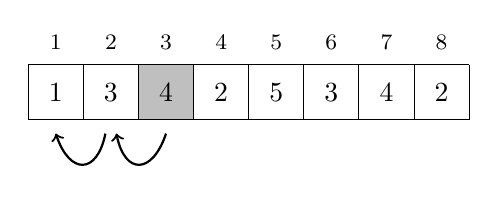
\begin{tikzpicture}[scale=0.7]
\fill[color=lightgray] (2,0) rectangle (3,1);
\draw (0,0) grid (8,1);

\node at (0.5,0.5) {$1$};
\node at (1.5,0.5) {$3$};
\node at (2.5,0.5) {$4$};
\node at (3.5,0.5) {$2$};
\node at (4.5,0.5) {$5$};
\node at (5.5,0.5) {$3$};
\node at (6.5,0.5) {$4$};
\node at (7.5,0.5) {$2$};

\draw[thick,->] (2.5,-0.25) .. controls (2.25,-1.00) and (1.75,-1.00) .. (1.6,-0.25);
\draw[thick,->] (1.4,-0.25) .. controls (1.25,-1.00) and (0.75,-1.00) .. (0.5,-0.25);

\footnotesize
\node at (0.5,1.4) {$1$};
\node at (1.5,1.4) {$2$};
\node at (2.5,1.4) {$3$};
\node at (3.5,1.4) {$4$};
\node at (4.5,1.4) {$5$};
\node at (5.5,1.4) {$6$};
\node at (6.5,1.4) {$7$};
\node at (7.5,1.4) {$8$};
\end{tikzpicture}
\end{center}

Taulukon seuraava luku 2 on pienempi kuin ketjun kaksi ensimmäistä lukua 4 ja 3.
Niinpä luvut 4 ja 3 poistetaan ketjusta, minkä jälkeen luku 2
lisätään ketjun alkuun. Sen lähin pienempi edeltäjä on luku 1:

\begin{center}
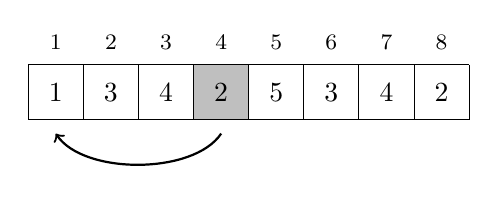
\begin{tikzpicture}[scale=0.7]
\fill[color=lightgray] (3,0) rectangle (4,1);
\draw (0,0) grid (8,1);

\node at (0.5,0.5) {$1$};
\node at (1.5,0.5) {$3$};
\node at (2.5,0.5) {$4$};
\node at (3.5,0.5) {$2$};
\node at (4.5,0.5) {$5$};
\node at (5.5,0.5) {$3$};
\node at (6.5,0.5) {$4$};
\node at (7.5,0.5) {$2$};

\draw[thick,->] (3.5,-0.25) .. controls (3.00,-1.00) and (1.00,-1.00) .. (0.5,-0.25);

\footnotesize
\node at (0.5,1.4) {$1$};
\node at (1.5,1.4) {$2$};
\node at (2.5,1.4) {$3$};
\node at (3.5,1.4) {$4$};
\node at (4.5,1.4) {$5$};
\node at (5.5,1.4) {$6$};
\node at (6.5,1.4) {$7$};
\node at (7.5,1.4) {$8$};
\end{tikzpicture}
\end{center}

Seuraava luku 5 on suurempi kuin luku 2,
joten se lisätään suoraan ketjun alkuun ja
sen lähin pienempi edeltäjä on luku 2:

\begin{center}
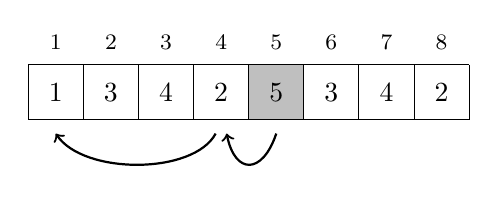
\begin{tikzpicture}[scale=0.7]
\fill[color=lightgray] (4,0) rectangle (5,1);
\draw (0,0) grid (8,1);

\node at (0.5,0.5) {$1$};
\node at (1.5,0.5) {$3$};
\node at (2.5,0.5) {$4$};
\node at (3.5,0.5) {$2$};
\node at (4.5,0.5) {$5$};
\node at (5.5,0.5) {$3$};
\node at (6.5,0.5) {$4$};
\node at (7.5,0.5) {$2$};

\draw[thick,->] (3.4,-0.25) .. controls (3.00,-1.00) and (1.00,-1.00) .. (0.5,-0.25);
\draw[thick,->] (4.5,-0.25) .. controls (4.25,-1.00) and (3.75,-1.00) .. (3.6,-0.25);

\footnotesize
\node at (0.5,1.4) {$1$};
\node at (1.5,1.4) {$2$};
\node at (2.5,1.4) {$3$};
\node at (3.5,1.4) {$4$};
\node at (4.5,1.4) {$5$};
\node at (5.5,1.4) {$6$};
\node at (6.5,1.4) {$7$};
\node at (7.5,1.4) {$8$};
\end{tikzpicture}
\end{center}

Algoritmi jatkaa samalla tavalla taulukon loppuun
ja selvittää jokaisen luvun lähimmän
pienemmän edeltäjän.
Mutta kuinka tehokas algoritmi on?

Algoritmin tehokkuus riippuu siitä,
kauanko ketjun käsittelyyn kuluu aikaa yhteensä.
Jos uusi luku on suurempi kuin ketjun ensimmäinen
luku, se vain lisätään ketjun alkuun,
mikä on tehokasta.
Joskus taas ketjussa voi olla useita
suurempia lukuja, joiden poistaminen vie aikaa.

Oleellista on kuitenkin, että jokainen
taulukossa oleva luku liittyy
tarkalleen kerran ketjuun ja poistuu
korkeintaan kerran ketjusta.
Niinpä jokainen luku aiheuttaa $O(1)$
ketjuun liittyvää operaatiota, ja tämän
seurauksena algoritmin kokonaisaikavaativuus on $O(n)$.

\section{Liukuvan ikkunan minimi}

\index{liukuvan ikkunan minimi@liukuvan ikkunan minimi}

\begin{task}
Annettuna on taulukko, jossa on $n$ lukua,
sekä kokonaisluku $k$.
Taulukon halki kulkee ikkuna, joka käy
läpi taulukon kaikki $k$-kokoiset välit.
Tehtäväsi on ilmoittaa jokaisesta ikkunasta
pienin välillä oleva luku.
\end{task}

Tämän tehtävän voi ratkaista lähes samalla
tavalla kuin edellisen tehtävän.
Ideana on pitää yllä ketjua, jonka alussa
on ikkunan viimeinen luku ja jossa jokainen
luku on edellistä pienempi. Joka vaiheessa
ketjun viimeinen luku on ikkunan pienin luku.

Kun liukuva ikkuna liikkuu eteenpäin ja välille
tulee uusi luku, ketjusta poistetaan kaikki luvut,
jotka ovat uutta lukua suurempia.
Tämän jälkeen uusi luku lisätään ketjun alkuun.
Lisäksi jos ketjun viimeinen luku ei enää kuulu
välille, se poistetaan ketjusta.

Tarkastellaan esimerkkinä, kuinka algoritmi selvittää
minimit seuraavassa taulukossa,
kun ikkunan koko $k=4$.

\begin{center}
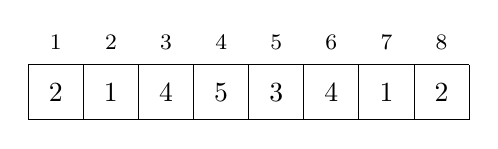
\begin{tikzpicture}[scale=0.7]
\draw (0,0) grid (8,1);

\node at (0.5,0.5) {$2$};
\node at (1.5,0.5) {$1$};
\node at (2.5,0.5) {$4$};
\node at (3.5,0.5) {$5$};
\node at (4.5,0.5) {$3$};
\node at (5.5,0.5) {$4$};
\node at (6.5,0.5) {$1$};
\node at (7.5,0.5) {$2$};

\footnotesize
\node at (0.5,1.4) {$1$};
\node at (1.5,1.4) {$2$};
\node at (2.5,1.4) {$3$};
\node at (3.5,1.4) {$4$};
\node at (4.5,1.4) {$5$};
\node at (5.5,1.4) {$6$};
\node at (6.5,1.4) {$7$};
\node at (7.5,1.4) {$8$};
\end{tikzpicture}
\end{center}

Liukuva ikkuna aloittaa matkansa taulukon vasemmasta reunasta.
Ensimmäisessä ikkunan sijainnissa pienin luku on 1:

\begin{center}
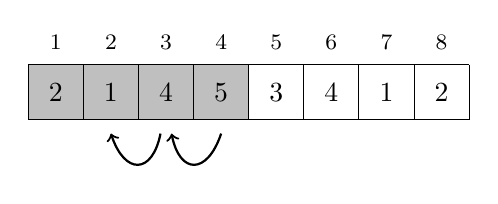
\begin{tikzpicture}[scale=0.7]
\fill[color=lightgray] (0,0) rectangle (4,1);
\draw (0,0) grid (8,1);

\node at (0.5,0.5) {$2$};
\node at (1.5,0.5) {$1$};
\node at (2.5,0.5) {$4$};
\node at (3.5,0.5) {$5$};
\node at (4.5,0.5) {$3$};
\node at (5.5,0.5) {$4$};
\node at (6.5,0.5) {$1$};
\node at (7.5,0.5) {$2$};

\footnotesize
\node at (0.5,1.4) {$1$};
\node at (1.5,1.4) {$2$};
\node at (2.5,1.4) {$3$};
\node at (3.5,1.4) {$4$};
\node at (4.5,1.4) {$5$};
\node at (5.5,1.4) {$6$};
\node at (6.5,1.4) {$7$};
\node at (7.5,1.4) {$8$};

\draw[thick,->] (3.5,-0.25) .. controls (3.25,-1.00) and (2.75,-1.00) .. (2.6,-0.25);
\draw[thick,->] (2.4,-0.25) .. controls (2.25,-1.00) and (1.75,-1.00) .. (1.5,-0.25);

\end{tikzpicture}
\end{center}

Kun ikkuna siirtyy eteenpäin, mukaan tulee luku 3,
joka on pienempi kuin luvut 5 ja 4 ketjun alussa.
Niinpä luvut 5 ja 4 poistuvat ketjusta ja luku 3
siirtyy sen alkuun. Pienin luku on edelleen 1.

\begin{center}
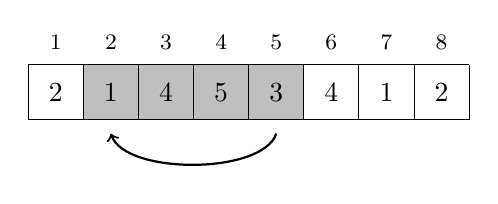
\begin{tikzpicture}[scale=0.7]
\fill[color=lightgray] (1,0) rectangle (5,1);
\draw (0,0) grid (8,1);

\node at (0.5,0.5) {$2$};
\node at (1.5,0.5) {$1$};
\node at (2.5,0.5) {$4$};
\node at (3.5,0.5) {$5$};
\node at (4.5,0.5) {$3$};
\node at (5.5,0.5) {$4$};
\node at (6.5,0.5) {$1$};
\node at (7.5,0.5) {$2$};

\footnotesize
\node at (0.5,1.4) {$1$};
\node at (1.5,1.4) {$2$};
\node at (2.5,1.4) {$3$};
\node at (3.5,1.4) {$4$};
\node at (4.5,1.4) {$5$};
\node at (5.5,1.4) {$6$};
\node at (6.5,1.4) {$7$};
\node at (7.5,1.4) {$8$};

\draw[thick,->] (4.5,-0.25) .. controls (4.25,-1.00) and (1.75,-1.00) .. (1.5,-0.25);

\end{tikzpicture}
\end{center}

Ikkuna siirtyy taas eteenpäin, jonka seurauksena pienin luku 1
putoaa pois ikkunasta. Niinpä se poistetaan ketjun lopusta
ja uusi pienin luku on 3. Lisäksi uusi ikkunaan tuleva luku 4
lisätään ketjun alkuun.

\begin{center}
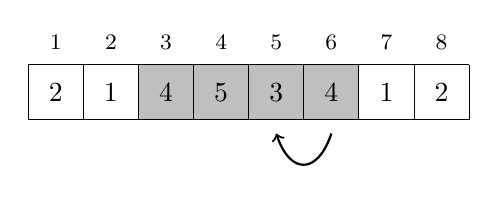
\begin{tikzpicture}[scale=0.7]
\fill[color=lightgray] (2,0) rectangle (6,1);
\draw (0,0) grid (8,1);

\node at (0.5,0.5) {$2$};
\node at (1.5,0.5) {$1$};
\node at (2.5,0.5) {$4$};
\node at (3.5,0.5) {$5$};
\node at (4.5,0.5) {$3$};
\node at (5.5,0.5) {$4$};
\node at (6.5,0.5) {$1$};
\node at (7.5,0.5) {$2$};

\footnotesize
\node at (0.5,1.4) {$1$};
\node at (1.5,1.4) {$2$};
\node at (2.5,1.4) {$3$};
\node at (3.5,1.4) {$4$};
\node at (4.5,1.4) {$5$};
\node at (5.5,1.4) {$6$};
\node at (6.5,1.4) {$7$};
\node at (7.5,1.4) {$8$};

\draw[thick,->] (5.5,-0.25) .. controls (5.25,-1.00) and (4.75,-1.00) .. (4.5,-0.25);
\end{tikzpicture}
\end{center}

Seuraavaksi ikkunaan tuleva luku 1 on pienempi
kuin kaikki ketjussa olevat luvut.
Tämän seurauksena koko ketju tyhjentyy ja
siihen jää vain luku 1:

\begin{center}
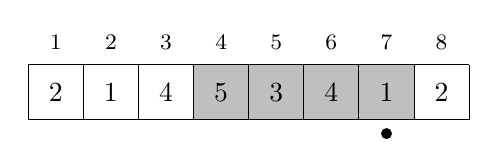
\begin{tikzpicture}[scale=0.7]
\fill[color=lightgray] (3,0) rectangle (7,1);
\draw (0,0) grid (8,1);

\node at (0.5,0.5) {$2$};
\node at (1.5,0.5) {$1$};
\node at (2.5,0.5) {$4$};
\node at (3.5,0.5) {$5$};
\node at (4.5,0.5) {$3$};
\node at (5.5,0.5) {$4$};
\node at (6.5,0.5) {$1$};
\node at (7.5,0.5) {$2$};

\footnotesize
\node at (0.5,1.4) {$1$};
\node at (1.5,1.4) {$2$};
\node at (2.5,1.4) {$3$};
\node at (3.5,1.4) {$4$};
\node at (4.5,1.4) {$5$};
\node at (5.5,1.4) {$6$};
\node at (6.5,1.4) {$7$};
\node at (7.5,1.4) {$8$};

\fill[color=black] (6.5,-0.25) circle (0.1);

%\draw[thick,->] (5.5,-0.25) .. controls (5.25,-1.00) and (4.75,-1.00) .. (4.5,-0.25);
\end{tikzpicture}
\end{center}

Lopuksi ikkuna saapuu viimeiseen sijaintiinsa.
Luku 2 lisätään ketjun alkuun,
mutta ikkunan pienin luku on edelleen 1.

\begin{center}
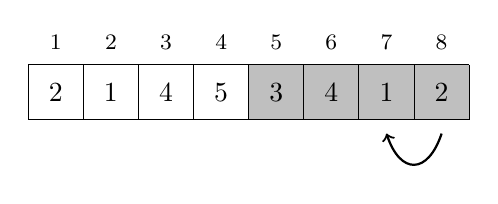
\begin{tikzpicture}[scale=0.7]
\fill[color=lightgray] (4,0) rectangle (8,1);
\draw (0,0) grid (8,1);

\node at (0.5,0.5) {$2$};
\node at (1.5,0.5) {$1$};
\node at (2.5,0.5) {$4$};
\node at (3.5,0.5) {$5$};
\node at (4.5,0.5) {$3$};
\node at (5.5,0.5) {$4$};
\node at (6.5,0.5) {$1$};
\node at (7.5,0.5) {$2$};

\footnotesize
\node at (0.5,1.4) {$1$};
\node at (1.5,1.4) {$2$};
\node at (2.5,1.4) {$3$};
\node at (3.5,1.4) {$4$};
\node at (4.5,1.4) {$5$};
\node at (5.5,1.4) {$6$};
\node at (6.5,1.4) {$7$};
\node at (7.5,1.4) {$8$};

\draw[thick,->] (7.5,-0.25) .. controls (7.25,-1.00) and (6.75,-1.00) .. (6.5,-0.25);
\end{tikzpicture}
\end{center}

Tässäkin algoritmissa jokainen taulukon luku lisätään
ketjuun tarkalleen kerran ja poistetaan ketjusta korkeintaan kerran,
joko ketjun alusta tai ketjun lopusta.
Niinpä algoritmin kokonaisaikavaativuus on $O(n)$.



